% Options for packages loaded elsewhere
\PassOptionsToPackage{unicode}{hyperref}
\PassOptionsToPackage{hyphens}{url}
%
\documentclass[
]{article}
\usepackage{amsmath,amssymb}
\usepackage{lmodern}
\usepackage{iftex}
\ifPDFTeX
  \usepackage[T1]{fontenc}
  \usepackage[utf8]{inputenc}
  \usepackage{textcomp} % provide euro and other symbols
\else % if luatex or xetex
  \usepackage{unicode-math}
  \defaultfontfeatures{Scale=MatchLowercase}
  \defaultfontfeatures[\rmfamily]{Ligatures=TeX,Scale=1}
\fi
% Use upquote if available, for straight quotes in verbatim environments
\IfFileExists{upquote.sty}{\usepackage{upquote}}{}
\IfFileExists{microtype.sty}{% use microtype if available
  \usepackage[]{microtype}
  \UseMicrotypeSet[protrusion]{basicmath} % disable protrusion for tt fonts
}{}
\makeatletter
\@ifundefined{KOMAClassName}{% if non-KOMA class
  \IfFileExists{parskip.sty}{%
    \usepackage{parskip}
  }{% else
    \setlength{\parindent}{0pt}
    \setlength{\parskip}{6pt plus 2pt minus 1pt}}
}{% if KOMA class
  \KOMAoptions{parskip=half}}
\makeatother
\usepackage{xcolor}
\IfFileExists{xurl.sty}{\usepackage{xurl}}{} % add URL line breaks if available
\IfFileExists{bookmark.sty}{\usepackage{bookmark}}{\usepackage{hyperref}}
\hypersetup{
  pdftitle={Assignment 2: Interpreting Quantitative Findings},
  hidelinks,
  pdfcreator={LaTeX via pandoc}}
\urlstyle{same} % disable monospaced font for URLs
\usepackage[margin=1in]{geometry}
\usepackage{graphicx}
\makeatletter
\def\maxwidth{\ifdim\Gin@nat@width>\linewidth\linewidth\else\Gin@nat@width\fi}
\def\maxheight{\ifdim\Gin@nat@height>\textheight\textheight\else\Gin@nat@height\fi}
\makeatother
% Scale images if necessary, so that they will not overflow the page
% margins by default, and it is still possible to overwrite the defaults
% using explicit options in \includegraphics[width, height, ...]{}
\setkeys{Gin}{width=\maxwidth,height=\maxheight,keepaspectratio}
% Set default figure placement to htbp
\makeatletter
\def\fps@figure{htbp}
\makeatother
\setlength{\emergencystretch}{3em} % prevent overfull lines
\providecommand{\tightlist}{%
  \setlength{\itemsep}{0pt}\setlength{\parskip}{0pt}}
\setcounter{secnumdepth}{5}
\newlength{\cslhangindent}
\setlength{\cslhangindent}{1.5em}
\newlength{\csllabelwidth}
\setlength{\csllabelwidth}{3em}
\newlength{\cslentryspacingunit} % times entry-spacing
\setlength{\cslentryspacingunit}{\parskip}
\newenvironment{CSLReferences}[2] % #1 hanging-ident, #2 entry spacing
 {% don't indent paragraphs
  \setlength{\parindent}{0pt}
  % turn on hanging indent if param 1 is 1
  \ifodd #1
  \let\oldpar\par
  \def\par{\hangindent=\cslhangindent\oldpar}
  \fi
  % set entry spacing
  \setlength{\parskip}{#2\cslentryspacingunit}
 }%
 {}
\usepackage{calc}
\newcommand{\CSLBlock}[1]{#1\hfill\break}
\newcommand{\CSLLeftMargin}[1]{\parbox[t]{\csllabelwidth}{#1}}
\newcommand{\CSLRightInline}[1]{\parbox[t]{\linewidth - \csllabelwidth}{#1}\break}
\newcommand{\CSLIndent}[1]{\hspace{\cslhangindent}#1}
\usepackage{amsmath}
\usepackage{booktabs}
\usepackage{lastpage}
\usepackage{fancyhdr}
\pagestyle{fancy}
\fancyhead{}
\renewcommand{\headrulewidth}{0pt}
\fancyfoot[CO,CE]{Page \thepage\ of \pageref{LastPage}}
\usepackage{floatrow}
\floatsetup[figure]{capposition=top}
\floatsetup[table]{capposition=top}
\usepackage{booktabs}
\usepackage{longtable}
\usepackage{array}
\usepackage{multirow}
\usepackage{wrapfig}
\usepackage{float}
\usepackage{colortbl}
\usepackage{pdflscape}
\usepackage{tabu}
\usepackage{threeparttable}
\usepackage{threeparttablex}
\usepackage[normalem]{ulem}
\usepackage{makecell}
\usepackage{xcolor}
\ifLuaTeX
  \usepackage{selnolig}  % disable illegal ligatures
\fi

\title{Assignment 2: Interpreting Quantitative Findings}
\usepackage{etoolbox}
\makeatletter
\providecommand{\subtitle}[1]{% add subtitle to \maketitle
  \apptocmd{\@title}{\par {\large #1 \par}}{}{}
}
\makeatother
\subtitle{\hfill\break
University of Glasgow\\
\strut \\
Student ID: 2819052\\
Course: Quantitative Methods\\
Number of words: 1076}
\author{}
\date{\vspace{-2.5em}}

\begin{document}
\maketitle

\pagebreak

\setcounter{tocdepth}{2}
\tableofcontents

\pagebreak

\hypertarget{introduction}{%
\section{Introduction}\label{introduction}}

In 1998, the Good Friday/Belfast Agreement was signed and later
validated by the voters, and this agreement marked a new era of hope
towards peace, equality, and inclusion in Northern Ireland
(\protect\hyperlink{ref-galligan2013gender}{Galligan 2013}). The main
focus on the agreement and referendum was obviously to stop the violent
conflict and seek peace, but one part of the agreement also emphasized
an equality agenda (\protect\hyperlink{ref-Hayward2021}{Hayward 2021}).
Thus, the agreement also marked the first Northern Irish formal
recognition of women's rights to political inclusion
(\protect\hyperlink{ref-galligan2013gender}{Galligan 2013}). However, a
formal recognition does not necessarily imply that gender equality
trickles down into social norms and practices. Therefore, this report
examines the contemporary state of women's equality in Northern Ireland.

Perhaps, the most central concept within gender equality is the
\emph{gender pay gap}. Disparities in income is an important indicator
for gender equality, because it has social, economic, and physiological
consequences (\protect\hyperlink{ref-bishu2017gender}{Bishu and Alkadry
2017}). Research on this area have identified several factors that seems
to influence a gender pay gap. One such factor can be inequality in
access to workplace authority, where women are denied manager or
supervisor position although there were equally qualified
(\protect\hyperlink{ref-bishu2017gender}{Bishu and Alkadry 2017}). Other
factors can be discrimination in hiring or promotion processes, but also
lack of gender representation can avoid minorities to even apply for a
job or promotion (\protect\hyperlink{ref-bishu2017gender}{Bishu and
Alkadry 2017}).

In order to examine the current gender equality in Northern Ireland, we
therefore focus on the gender pay gap in Northern Ireland. We ask the
following research question: \emph{Does gender affect income in
contemporary Northern Ireland?} We employ a deductive approach, where we
first formulate a hypothesis and subsequently examine it empirically
(\protect\hyperlink{ref-bryman2016social}{Bryman 2016, 33}). Therefore,
our analysis consider the following null hypothesis (H\textsubscript{0})
and alternative hypothesis (H\textsubscript{A}):

\begin{itemize}
\tightlist
\item
  H\textsubscript{0}: Being a woman or man does not affect your income.
\item
  H\textsubscript{A}: Being a woman rather than a man affects a lower
  income.
\end{itemize}

The causal relationship that we examine is thus a negative relationship.
Although, we call this relationship causal, it is important to clarify
that I do not imply that there is anything biological or deterministic
that reduce women's income in general. Rather, the causal link is
interpreted as a result of the societal discriminatory practices
explained in the previous paragraph. To make a convincing inquiry of
this causal relationship, we must also control for a number of other
factor related to income and gender. This is important to make sure that
our analysis do not simply show a spurious correlation as it could in
fact be another factor that influences both gender and income. These
control variables are introduced in the Data and Methods-section.

\hypertarget{data-and-method}{%
\section{Data and method}\label{data-and-method}}

The research design of this analysis is a cross-sectional design
(\protect\hyperlink{ref-bryman2016social}{Bryman 2016, 53}). This means
that the data for analysis is collected at a single point in time and
consists of a sample of respondents from which we seek to infer to a
general population of Northern Ireland
(\protect\hyperlink{ref-field2012discovering}{Field, Miles, and Field
2012, 36}). This section describes this sample and how the data was
collected, and then subsequently the operationalized variables to
examine our research hypothesis are described.

\hypertarget{sample-and-data-collection}{%
\subsection{Sample and Data
Collection}\label{sample-and-data-collection}}

Our sample for the analysis consists of data from Northern Ireland Life
and Times Survey (NILT). The data have been collected every year since
1998, but this analysis uses the survey from 2012
(\protect\hyperlink{ref-ark_2012}{ARK 2012}). The respondents for the
NILT survey was chosen from a systematic random sample of addresses.
From this sample of 2126 addresses, 1204 questionnaires were fully
completed using partly face-to-face- and self-completion questionnaires
(\protect\hyperlink{ref-ark_2012}{ARK 2012}). Our sample of analysis is
further reduced as not all respondents have answered our variables of
interest, and we are therefore not able to include those respondents in
our analysis. In the tables below, we present descriptive statistics for
our variables of interest in both the full NILT sample and our sample of
analysis. The first tables shows the categorical variables, where a
frequency distribution are shown
(\protect\hyperlink{ref-fogarty2018quantitative}{Fogarty 2018, 88}). The
second table shows the numerical variables, where we have calculated the
mean and standard deviation
(\protect\hyperlink{ref-fogarty2018quantitative}{Fogarty 2018, 95}).

\begin{table}[H]

\caption{\label{tab:unnamed-chunk-1}Descriptive Statistics for Cleaned and Full Sample (Categorical Variables)}
\centering
\begin{tabular}[t]{llllll}
\toprule
\multicolumn{1}{c}{ } & \multicolumn{2}{c}{Cleaned Sample} & \multicolumn{2}{c}{Full Sample} & \multicolumn{1}{c}{ } \\
\cmidrule(l{3pt}r{3pt}){2-3} \cmidrule(l{3pt}r{3pt}){4-5}
Variable & N & Percent & N & Percent & Test\\
\midrule
Sex & 675 &  & 1204 &  & X2=1.022\\
... Male & 284 & 42.1\% & 537 & 44.6\% & \\
... Female & 391 & 57.9\% & 667 & 55.4\% & \\
Religion & 675 &  & 1168 &  & X2=0.849\\
... Catholic & 277 & 41\% & 491 & 42\% & \\
\addlinespace
... Protestant & 283 & 41.9\% & 497 & 42.6\% & \\
... No religion & 115 & 17\% & 180 & 15.4\% & \\
Sexual Orientation & 675 &  & 1191 &  & X2=3.039\\
... I am heterosexual or straight & 657 & 97.3\% & 1173 & 98.5\% & \\
... I am gay or lesbian (homosexual) & 14 & 2.1\% & 14 & 1.2\% & \\
\addlinespace
... I am bi-sexual & 2 & 0.3\% & 2 & 0.2\% & \\
... Other & 2 & 0.3\% & 2 & 0.2\% & \\
Constitutional View & 675 &  & 1183 &  & X2=0.347\\
... Unionist & 199 & 29.5\% & 348 & 29.4\% & \\
... Nationalist & 138 & 20.4\% & 255 & 21.6\% & \\
\addlinespace
... Neither & 338 & 50.1\% & 580 & 49\% & \\
Trade union membership & 675 &  & 1179 &  & X2=9.162***\\
... Yes & 301 & 44.6\% & 440 & 37.3\% & \\
... No & 374 & 55.4\% & 739 & 62.7\% & \\
Supervisor: No & 675 &  & 883 &  & X2=0.143\\
\addlinespace
... Yes & 211 & 31.3\% & 267 & 30.2\% & \\
... No & 464 & 68.7\% & 616 & 69.8\% & \\
\bottomrule
\multicolumn{6}{l}{\rule{0pt}{1em}\textit{Note: }}\\
\multicolumn{6}{l}{\rule{0pt}{1em}Statistical significance markers: * p<0.1; ** p<0.05; *** p<0.01}\\
\end{tabular}
\end{table}

\begin{table}[H]

\caption{\label{tab:unnamed-chunk-1}Descriptive Statistics for Cleaned and Full Sample (Numerical Variables)}
\centering
\begin{tabular}[t]{llllllll}
\toprule
\multicolumn{1}{c}{ } & \multicolumn{3}{c}{Cleaned Sample} & \multicolumn{3}{c}{Full Sample} & \multicolumn{1}{c}{ } \\
\cmidrule(l{3pt}r{3pt}){2-4} \cmidrule(l{3pt}r{3pt}){5-7}
Variable & N & Mean & SD & N & Mean & SD & Test\\
\midrule
Annual Personal Income (GBP) & 675 & 16892.089 & 13447.704 & 897 & 16394.582 & 13465.9 & F=0.526\\
Age & 675 & 46.763 & 17.117 & 1201 & 49.615 & 18.53 & F=10.81***\\
\bottomrule
\multicolumn{8}{l}{\rule{0pt}{1em}\textit{Note: }}\\
\multicolumn{8}{l}{\rule{0pt}{1em}Statistical significance markers: * p<0.1; ** p<0.05; *** p<0.01}\\
\end{tabular}
\end{table}

In the table with categorical variables, we conduct a Chi-squared test
to check if there is independence between the samples or not,
i.e.~whether the frequency distribution is significantly different
(\protect\hyperlink{ref-fogarty2018quantitative}{Fogarty 2018, 176}).
For the numerical variables, we conduct an Analysis of Variances (ANOVA)
to test whether the means in the two samples are significantly different
(\protect\hyperlink{ref-field2012discovering}{Field, Miles, and Field
2012, 399ff}). For the categorical variables, we see that for the test
of trade union membership, the test value is 9.162, which is
significantly different from 0 (with a p-value less than 0.01). This
indicates that the frequency distribution in our sample is significantly
different from the full NILT sample. There is a larger share (44.6 \%)
of members of a trade union after removing missing values compared to
only 37.3 \% in the full NILT sample. Similarly, we see from the ANOVA
that the test value (F) for age is significantly different from 0 (with
a p-value less than 0.01) meaning that our sample is different from the
full NILT sample in the age distribution. We can see that the mean age
is only around 46 years compared to 49 years in the full NILT sample.
These two findings are important to bear in mind, when we interpret our
final conclusion as both age and trade union membership might be related
to our dependent variable, income.

The systematic random sampling strategy in the NILT survey is an
approach to make the sample representative of our population - in our
case all inhabitants of Northern Ireland. It could be relevant to
examine the demographic distribution in our sample against the general
population of Northern Ireland, but unfortunately that is beyond the
scope of this report.

\hypertarget{dependent-independent-and-control-variables}{%
\subsection{Dependent, Independent, and Control
Variables}\label{dependent-independent-and-control-variables}}

Levels of measurement: nominal, ordinal, interval, and ratio
(\protect\hyperlink{ref-fogarty2018quantitative}{Fogarty 2018, 56})

\begin{figure}[H]

{\centering 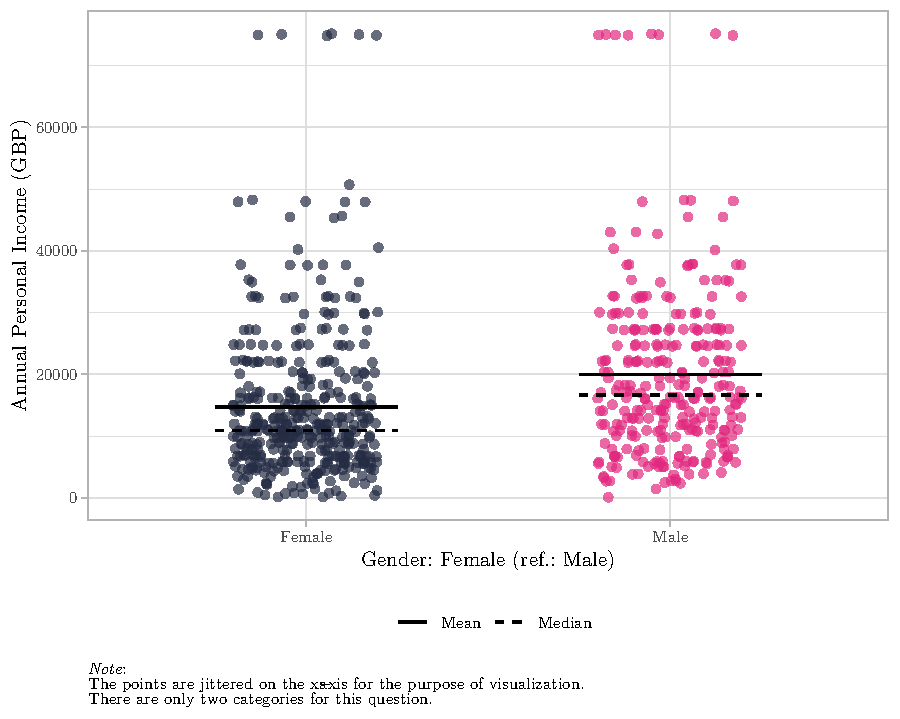
\includegraphics[width=0.8\linewidth]{paper_files/figure-latex/unnamed-chunk-2-1} 

}

\caption{Scatterplot of Income and Sex}\label{fig:unnamed-chunk-2}
\end{figure}

To fully examine the relationship between our dependent and independent
variable, we employ a multiple linear regression estimated with OLS
{[}fogarty2018quantitative 192ff{]}. Thus, we are also able to include
the control variables to make the acceptance or decline of our
hypothesis more convincing.

\hypertarget{results-and-discussion}{%
\section{Results and discussion}\label{results-and-discussion}}

Here comes the regression.

\begin{table}[H] \centering 
  \caption{Regression results} 
  \label{} 
\small 
\begin{tabular}{@{\hspace{5pt}}l@{\hspace{5pt}}c} 
\toprule 
 & \multicolumn{1}{c}{Dependent Variable} \\ 
\cmidrule(rr){2-2} 
 & Annual Personal Income (GBP) \\ 
\midrule  
\\[-2.1ex] Sex: Female (ref.: Male) & $-$5,068.737$^{***}$ \\ 
  & (994.748) \\ 
 \addlinespace 
 Religion: Protestant (ref.: Catholic) & 465.188 \\ 
  & (1,458.367) \\ 
 \addlinespace 
 Religion: No religion & 895.169 \\ 
  & (1,533.323) \\ 
 \addlinespace 
 Sexual Orientation: Homosexual (ref.: Heterosexual) & $-$6,247.777$^{*}$ \\ 
  & (3,437.048) \\ 
 \addlinespace 
 Sexual Orientation: bi-sexual & $-$2,826.980 \\ 
  & (8,698.806) \\ 
 \addlinespace 
 Sexual Orientation: Other & 1,323.336 \\ 
  & (8,737.282) \\ 
 \addlinespace 
 Constitutional View: Nationalist (ref.: Unionist) & 1,788.873 \\ 
  & (1,898.294) \\ 
 \addlinespace 
 Constitutional view: Neither & 1,438.036 \\ 
  & (1,350.423) \\ 
 \addlinespace 
 Trade union membership: No (ref.: Yes) & $-$5,277.978$^{***}$ \\ 
  & (977.008) \\ 
 \addlinespace 
 Supervisor: No (ref.: Yes) & $-$8,648.320$^{***}$ \\ 
  & (1,037.559) \\ 
 \addlinespace 
 Age & $-$84.369$^{***}$ \\ 
  & (29.430) \\ 
 \addlinespace 
 Constant & 31,343.540$^{***}$ \\ 
  & (2,488.067) \\ 
 \addlinespace 
\midrule  
Observations & 675 \\ 
R$^{2}$ & 0.183 \\ 
Adjusted R$^{2}$ & 0.170 \\ 
Residual Std. Error & 12,252.840 (df = 663) \\ 
F Statistic & 13.533$^{***}$ (df = 11; 663) \\ 
\bottomrule 
\textit{Note:}  & \multicolumn{1}{r}{$^{*}$p$<$0.1; $^{**}$p$<$0.05; $^{***}$p$<$0.01} \\ 
\end{tabular} 
\end{table}

Effect sizes (\protect\hyperlink{ref-field2012discovering}{Field, Miles,
and Field 2012, 57}) Influential data points / outliers
(\protect\hyperlink{ref-fogarty2018quantitative}{Fogarty 2018, 221--22})

\hypertarget{check-for-heteroscedasticity}{%
\subsection{Check for
Heteroscedasticity}\label{check-for-heteroscedasticity}}

Here comes a check for heteroscedasticity.

\begin{figure}[H]

{\centering 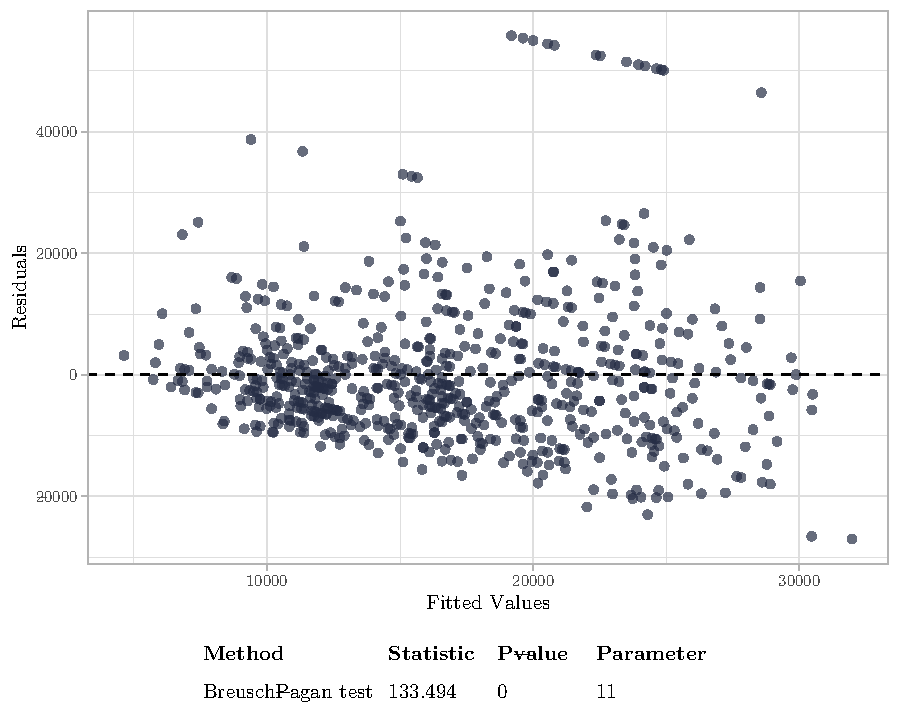
\includegraphics[width=0.8\linewidth]{paper_files/figure-latex/unnamed-chunk-4-1} 

}

\caption{Scatterplot of Fitted Values and Residuals}\label{fig:unnamed-chunk-4}
\end{figure}

\hypertarget{reliability-and-validity}{%
\subsection{Reliability and Validity}\label{reliability-and-validity}}

Reliability and validity
(\protect\hyperlink{ref-bryman2016social}{Bryman 2016, 41}) Internal and
external validity (\protect\hyperlink{ref-bryman2016social}{Bryman 2016,
41--42})

\hypertarget{conclusion}{%
\section{Conclusion}\label{conclusion}}

\pagebreak

\hypertarget{references}{%
\section{References}\label{references}}

\hypertarget{refs}{}
\begin{CSLReferences}{1}{0}
\leavevmode\vadjust pre{\hypertarget{ref-ark_2012}{}}%
ARK. 2012. \emph{2012 Northern Ireland Life \&Amp; Times Survey:
Technical Notes}. ARK. \url{https://www.ark.ac.uk/nilt/2012/tech12.pdf}.

\leavevmode\vadjust pre{\hypertarget{ref-bishu2017gender}{}}%
Bishu, Sebawit G., and Mohamad G. Alkadry. 2017. {``A Systematic Review
of the Gender Pay Gap and Factors That Predict It.''}
\emph{Administration \& Society} 49 (1): 65--104.
\url{https://doi.org/10.1177/0095399716636928}.

\leavevmode\vadjust pre{\hypertarget{ref-bryman2016social}{}}%
Bryman, A. 2016. \emph{Social Research Methods}. Oxford University
Press. \url{https://books.google.co.uk/books?id=N2zQCgAAQBAJ}.

\leavevmode\vadjust pre{\hypertarget{ref-field2012discovering}{}}%
Field, A., J. Miles, and Z. Field. 2012. \emph{Discovering Statistics
Using r}. SAGE Publications.
\url{https://books.google.co.uk/books?id=wd2K2zC3swIC}.

\leavevmode\vadjust pre{\hypertarget{ref-fogarty2018quantitative}{}}%
Fogarty, B. J. 2018. \emph{Quantitative Social Science Data with r: An
Introduction}. Core Textbook. SAGE Publications.
\url{https://books.google.co.uk/books?id=jwJ6DwAAQBAJ}.

\leavevmode\vadjust pre{\hypertarget{ref-galligan2013gender}{}}%
Galligan, Yvonne. 2013. {``Gender and Politics in Northern Ireland: The
Representation Gap Revisited.''} \emph{Irish Political Studies} 28 (3):
413--33.

\leavevmode\vadjust pre{\hypertarget{ref-Hayward2021}{}}%
Hayward, Katy. 2021. {``The 1998 Good Friday (Belfast) Agreement
Referendums in Northern Ireland and the Republic of Ireland.''} In
\emph{The Palgrave Handbook of European Referendums}, edited by Julie
Smith, 247--65. Cham: Springer International Publishing.
\url{https://doi.org/10.1007/978-3-030-55803-1_12}.

\end{CSLReferences}

\pagebreak

\hypertarget{appendix}{%
\section{Appendix}\label{appendix}}

\begin{figure}[H]

{\centering 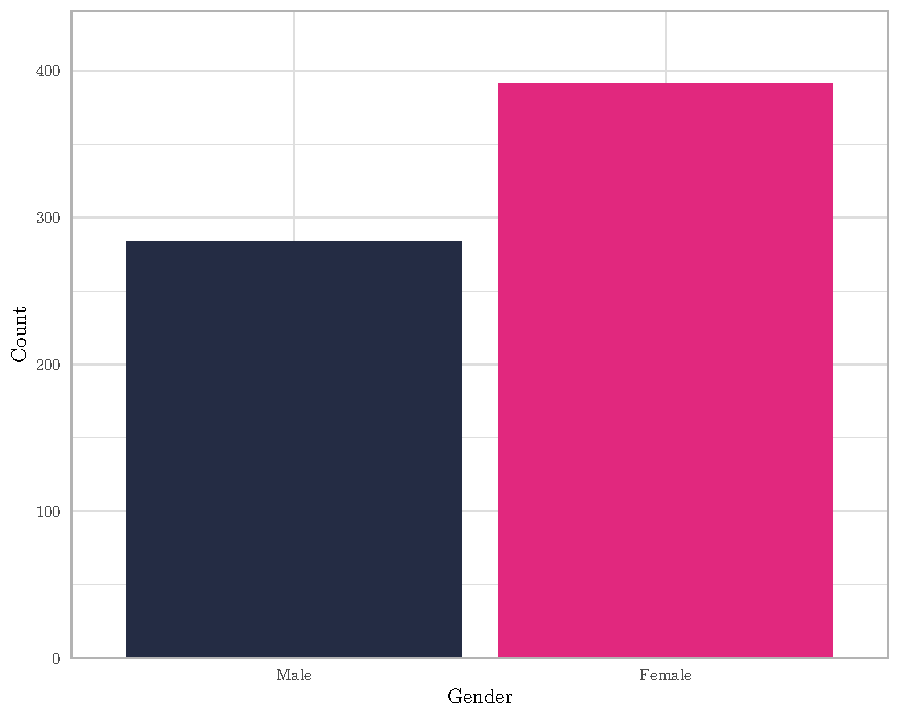
\includegraphics[width=0.8\linewidth]{paper_files/figure-latex/unnamed-chunk-5-1} 

}

\caption{Barplot of Sex}\label{fig:unnamed-chunk-5}
\end{figure}

\begin{figure}[H]

{\centering 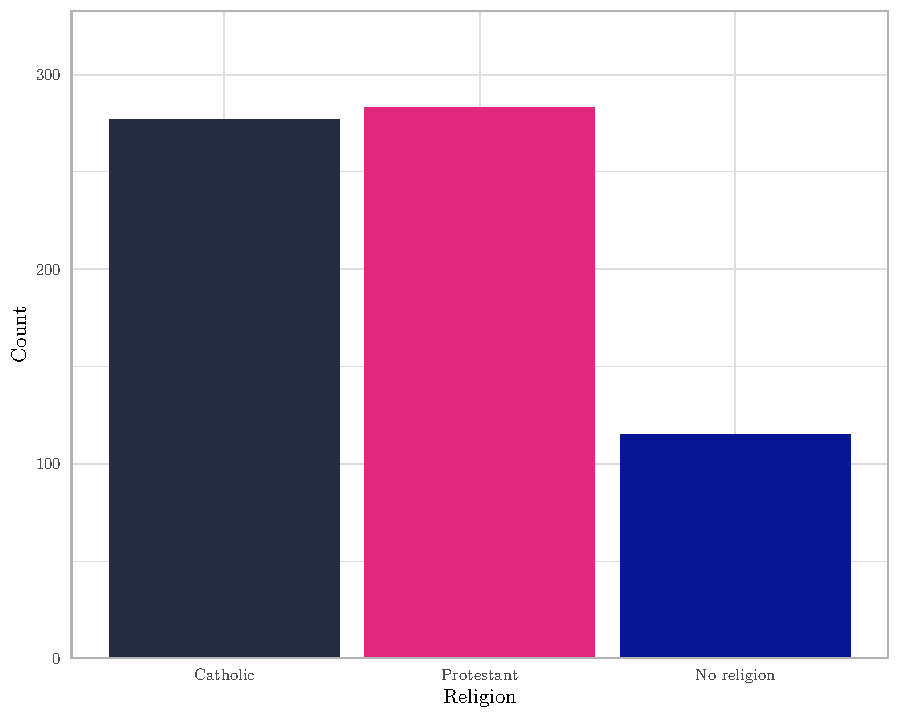
\includegraphics[width=0.8\linewidth]{paper_files/figure-latex/unnamed-chunk-6-1} 

}

\caption{Barplot of Religion}\label{fig:unnamed-chunk-6}
\end{figure}

\begin{figure}[H]

{\centering 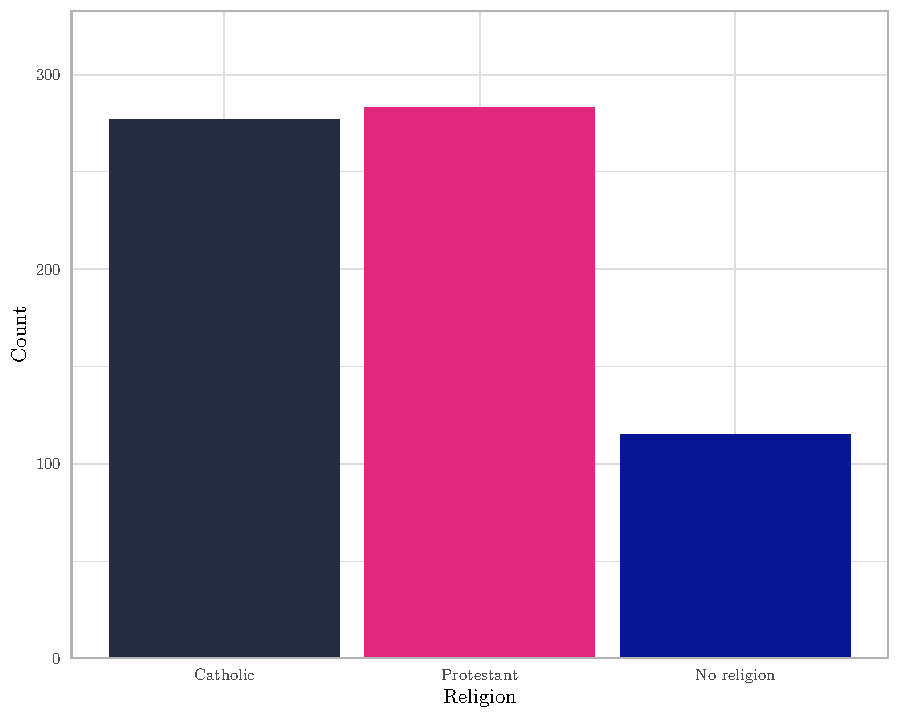
\includegraphics[width=0.8\linewidth]{paper_files/figure-latex/unnamed-chunk-7-1} 

}

\caption{Barplot of Sexual Orientation}\label{fig:unnamed-chunk-7}
\end{figure}

\begin{figure}[H]

{\centering 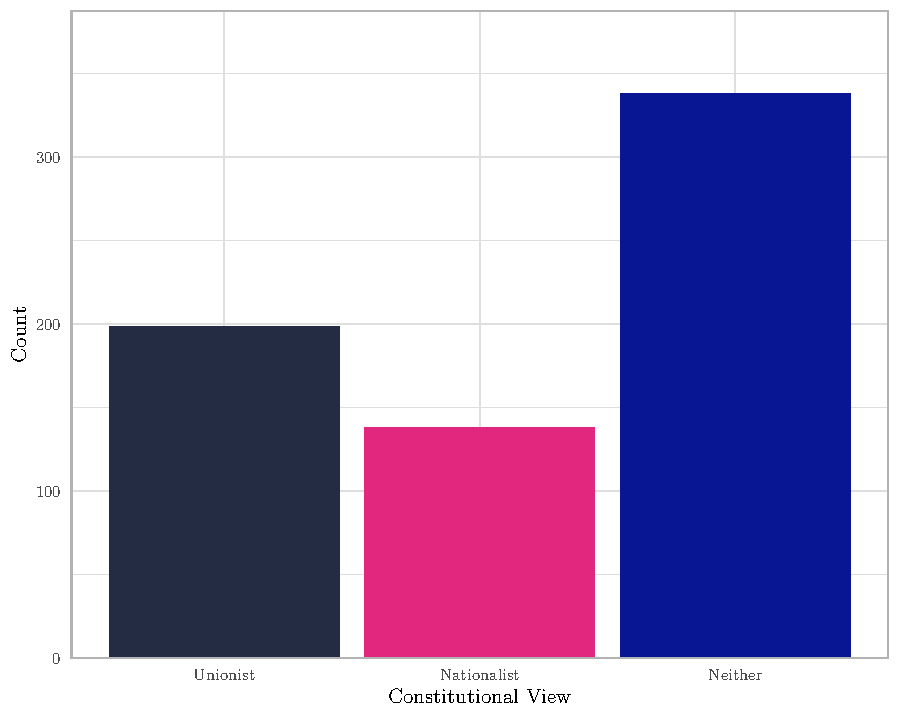
\includegraphics[width=0.8\linewidth]{paper_files/figure-latex/unnamed-chunk-8-1} 

}

\caption{Barplot of Constitutional View}\label{fig:unnamed-chunk-8}
\end{figure}

\begin{figure}[H]

{\centering 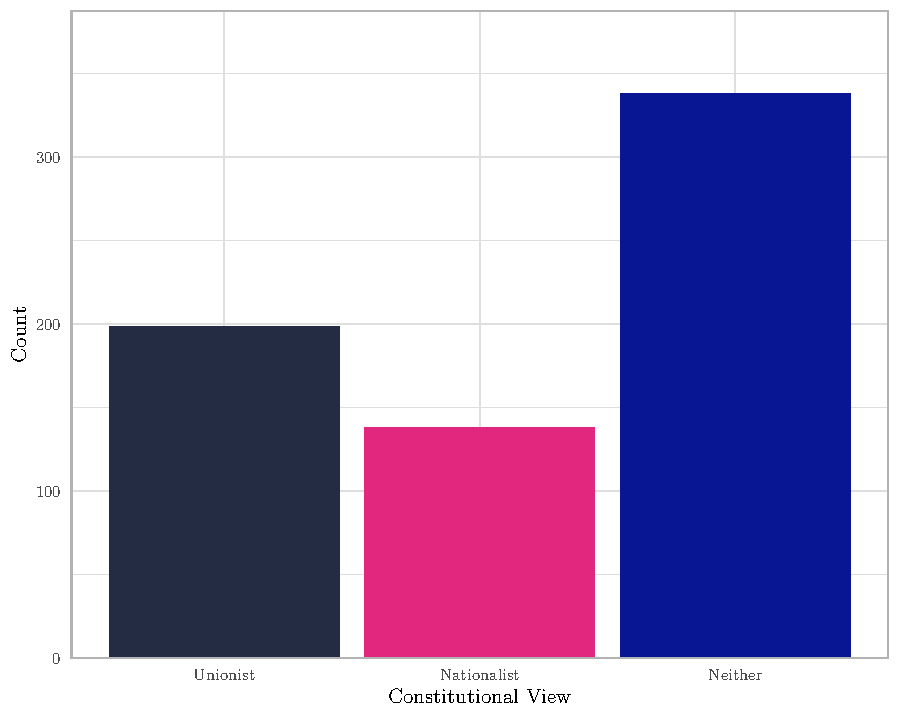
\includegraphics[width=0.8\linewidth]{paper_files/figure-latex/unnamed-chunk-9-1} 

}

\caption{Barplot of Trade union membership}\label{fig:unnamed-chunk-9}
\end{figure}

\begin{figure}[H]

{\centering 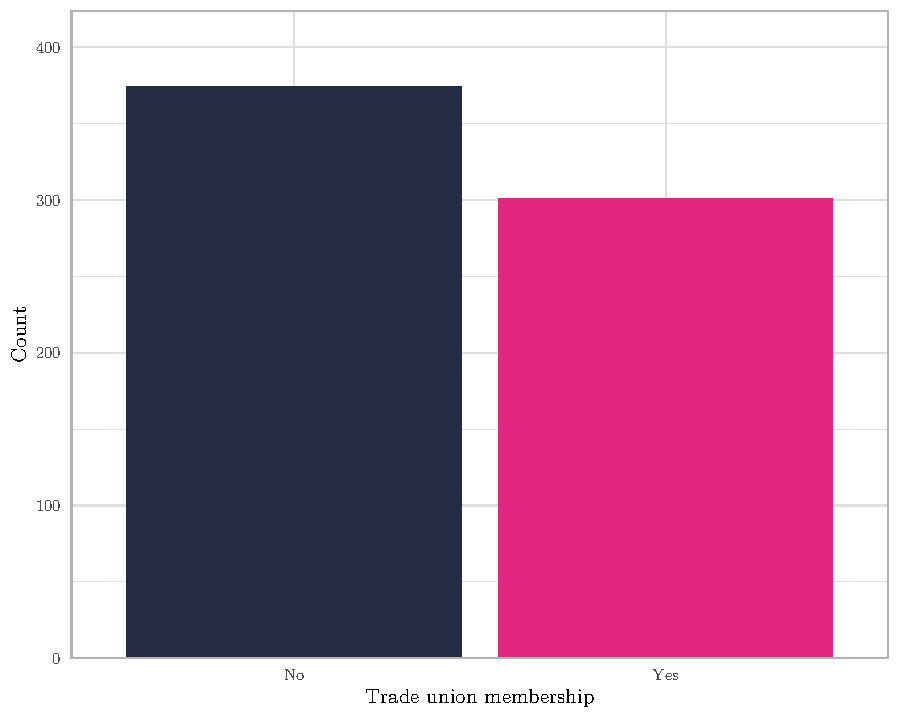
\includegraphics[width=0.8\linewidth]{paper_files/figure-latex/unnamed-chunk-10-1} 

}

\caption{Barplot of Supervisor}\label{fig:unnamed-chunk-10}
\end{figure}

\begin{figure}[H]

{\centering 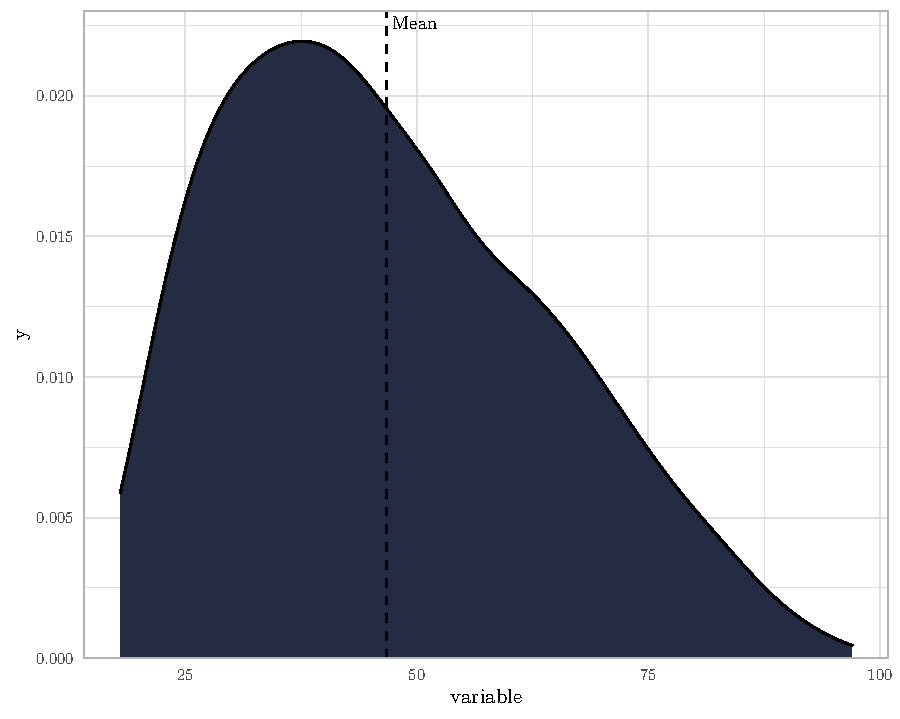
\includegraphics[width=0.8\linewidth]{paper_files/figure-latex/unnamed-chunk-11-1} 

}

\caption{Density plot of Age}\label{fig:unnamed-chunk-11}
\end{figure}

\begin{figure}[H]

{\centering 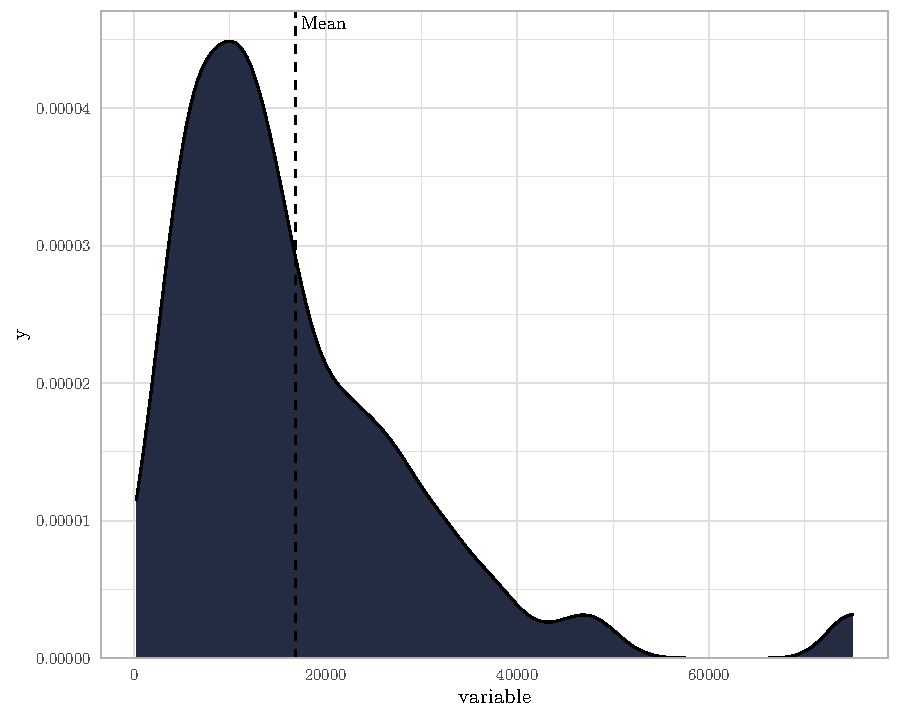
\includegraphics[width=0.8\linewidth]{paper_files/figure-latex/unnamed-chunk-12-1} 

}

\caption{Density plot of Income}\label{fig:unnamed-chunk-12}
\end{figure}

\end{document}
